\section{Question 2}
In this question, we investigate the effect of perturbation forces on the orbital elements.
\subsection{$J_2$ perturbation}

Forces in RSW system:
\begin{equation}
    \begin{aligned}
        F_R = & -\dfrac{3\mu J_2 R^2}{2r^4}\left(1-3\sin^2(i)\sin^2(u_0)\right)\\
        F_S = & -\dfrac{3\mu J_2 R^2}{2r^4}\sin^2(i)\sin(u_0)\cos(u_0)\\
        F_W = & -\dfrac{3\mu J_2 R^2}{2r^4}\sin(i)\cos(i)\sin(u_0)
    \end{aligned}
\end{equation}
From \eqref{eq:all_perturbation_equations} we know the effect of other forces on orbital elements. Here is the result of perturbation forces on orbital elements.
The simulation has been in the Jupyter notebook. the results are presented here.
\begin{figure}[H]
    \centering
    \includegraphics[width=0.85\textwidth]{../Figure/Q2/orbital_elements_100.pdf}
    \caption{Variation of Parameter due to $J_2$ perturbation for 100 seconds}
\end{figure}

\begin{figure}[H]
    \centering
    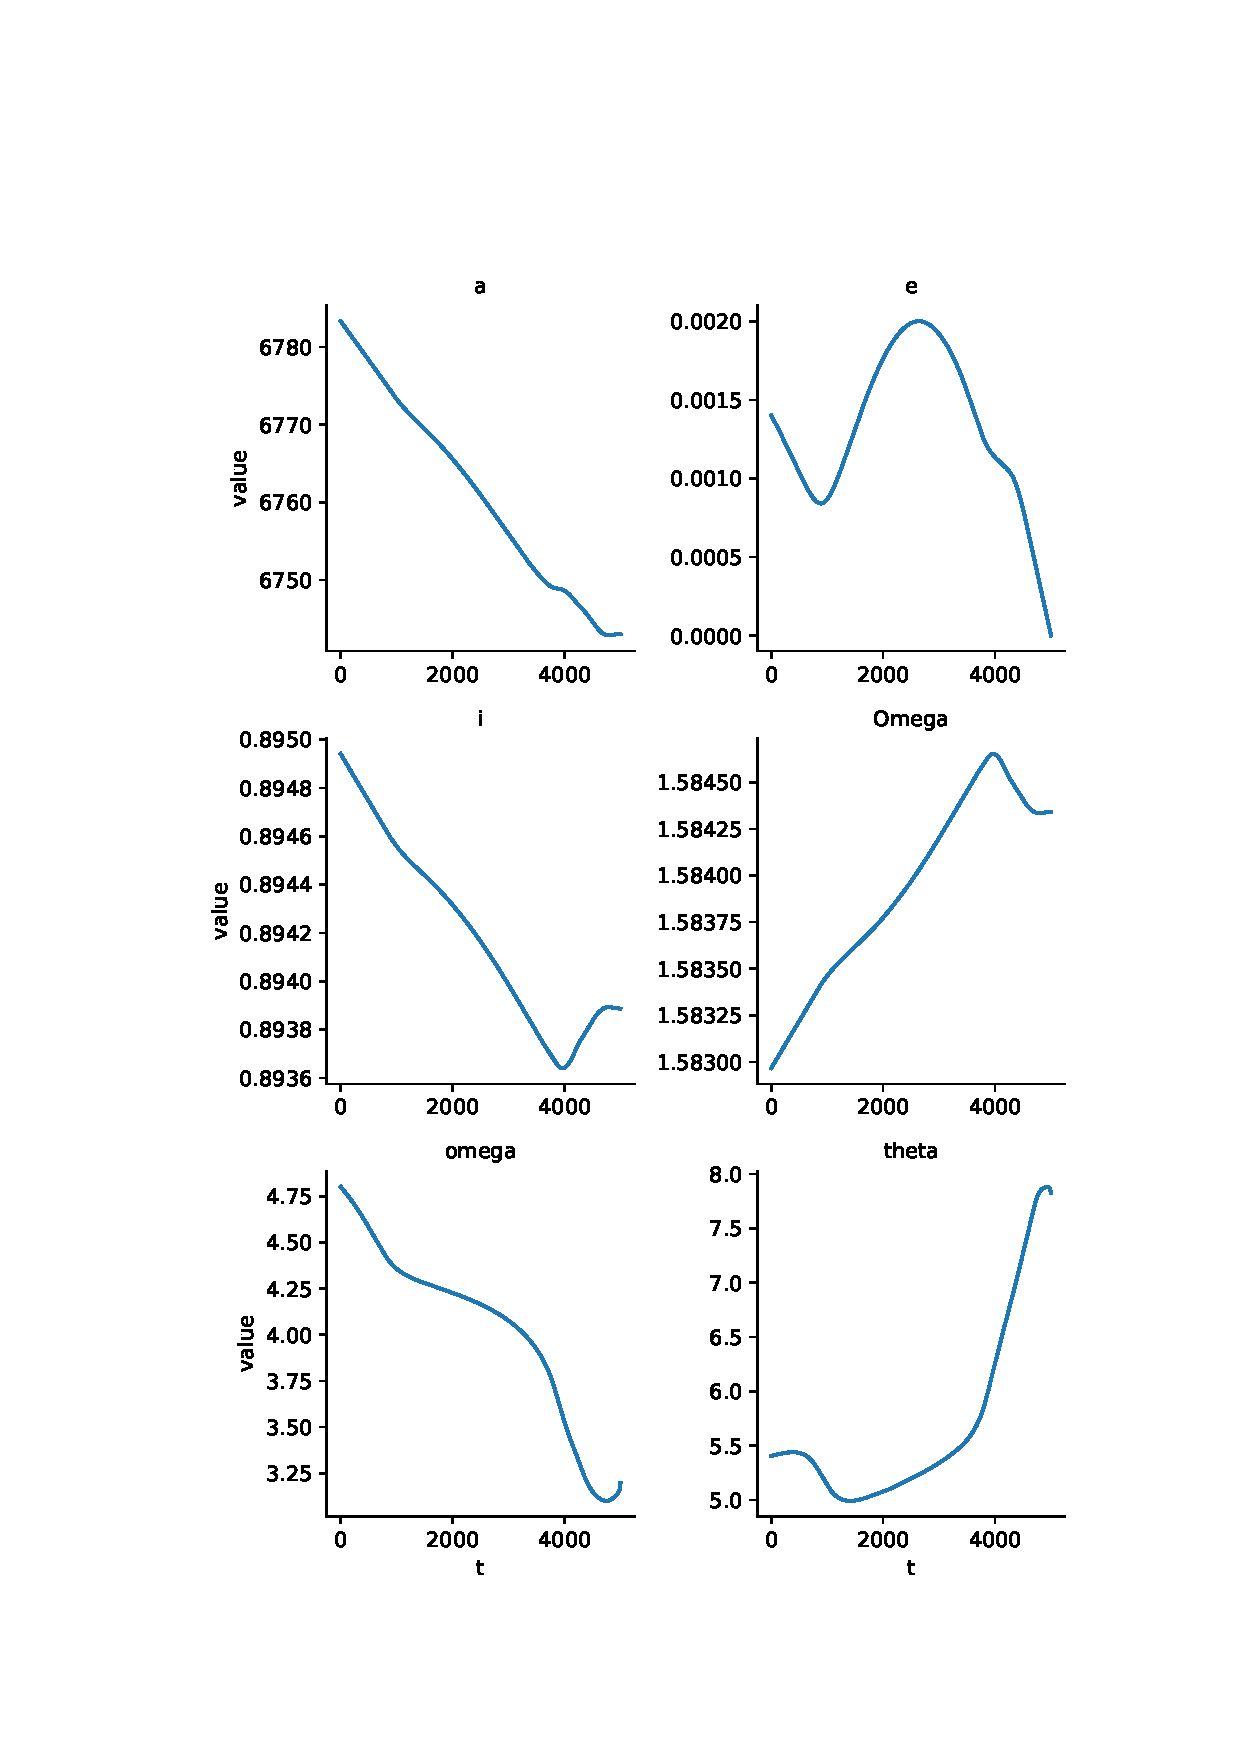
\includegraphics[width=0.85\textwidth]{../Figure/Q2/orbital_elements_5000.pdf}
    \caption{Variation of Parameter due to $J_2$ perturbation for 5000 seconds}
\end{figure}

\begin{figure}[H]
    \centering
    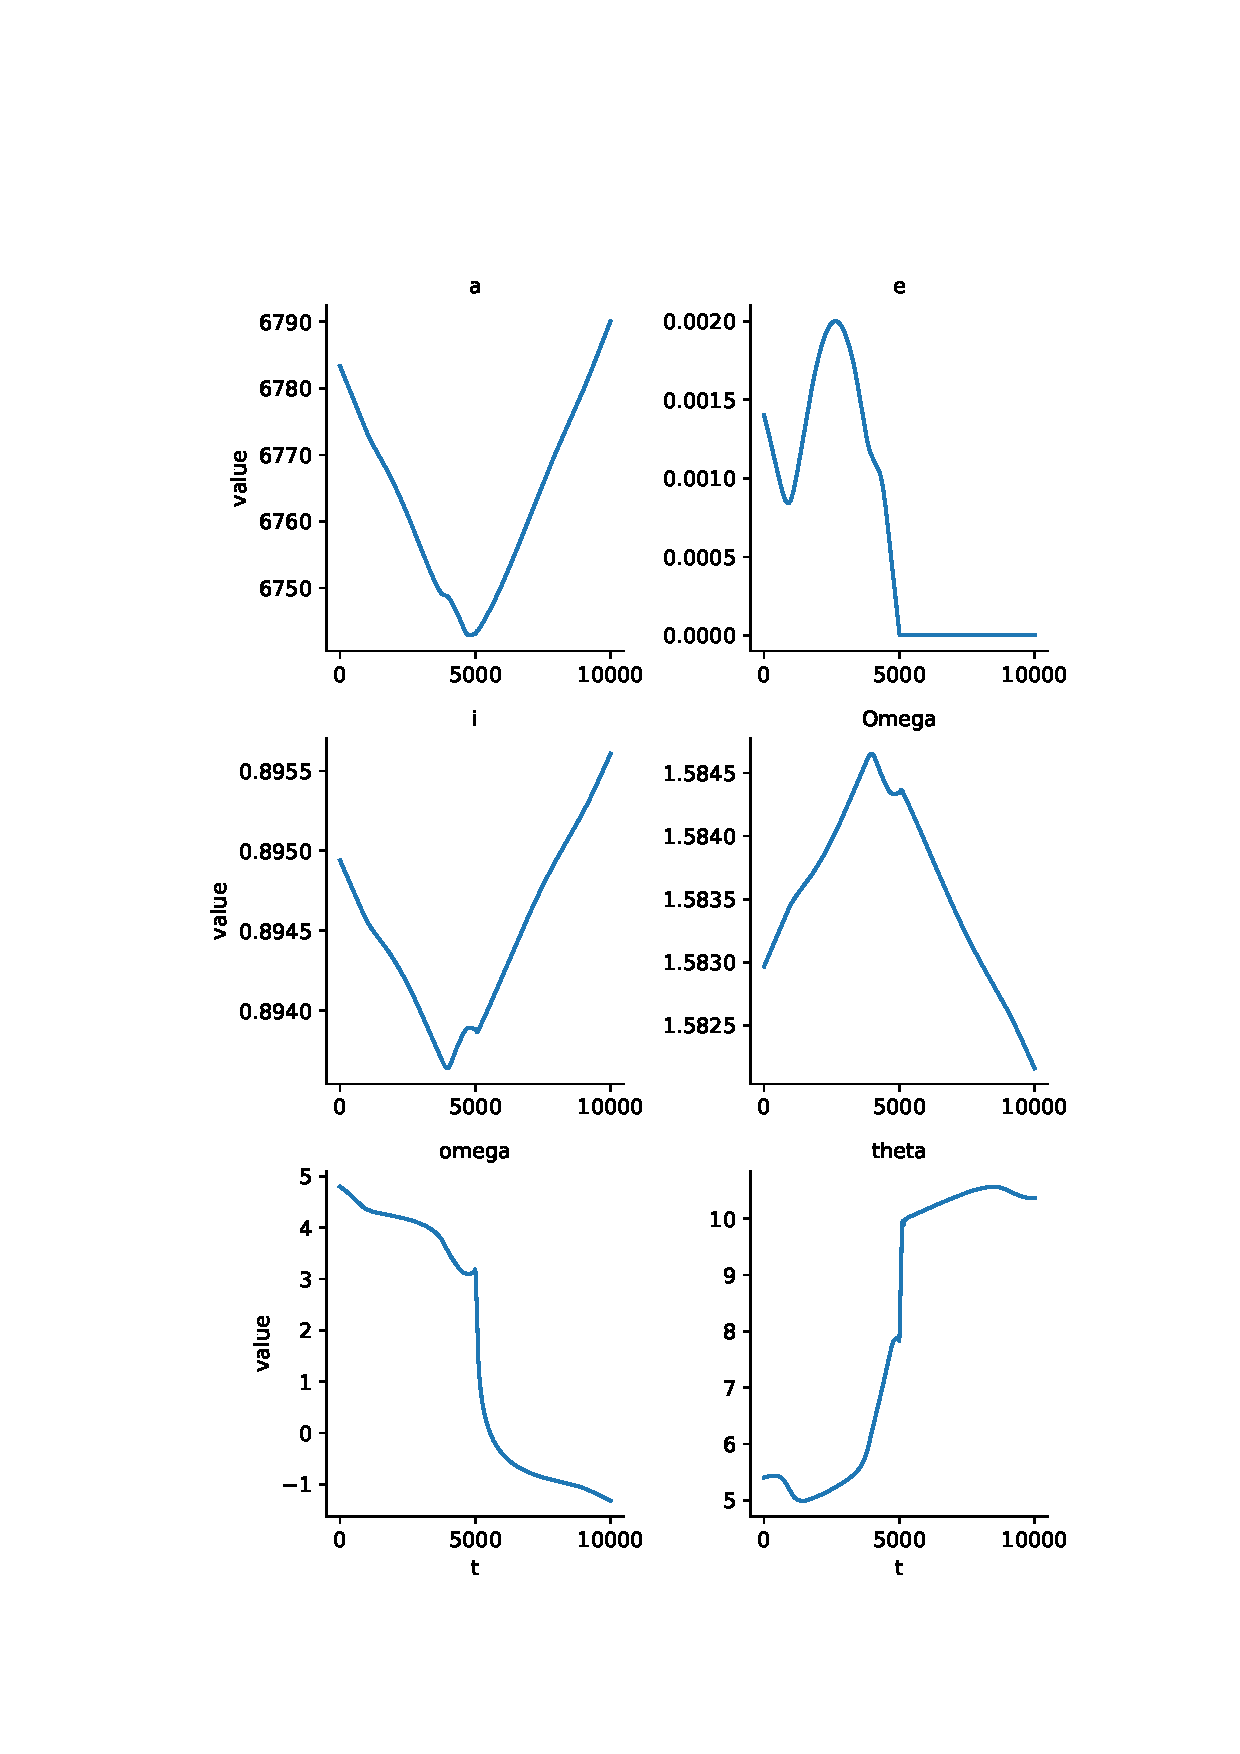
\includegraphics[width=0.85\textwidth]{../Figure/Q2/orbital_elements_10000.pdf}
    \caption{Variation of Parameter due to $J_2$ perturbation for 10000 seconds}
\end{figure}